\clearpage
\section{Design, Development and Evaluation}
\label{sec:TADF/development}
Turning the foundations of Chapter~\ref{sec:Background} into decision support takes four steps: objectives, evidence, design and evaluation. This chapter reports these steps for the TADF.  Section~\ref{subsec:TADF/objectives} derives eight design objectives. Section~\ref{subsec:TADF/design} reports the experimental program that compared both orchestration paradigms on the same tasks. Section~\ref{subsec:TADF/initial-artifact} presents the initial framework, the Decision Sheet, and shows how this evidence shaped its gates and scoring rules. Section~\ref{subsec:TADF/evaluation} reports two evaluation episodes: practitioner interviews and a WorkBench evaluation. It also describes the revisions they caused and two pilot runs of the revised framework. Because they were highly formative, they are reported together with the design and devleopment \parencite{gregorPositioningPresentingDesign2013}.

\subsection{Design Objectives for the Framework}
\label{subsec:TADF/objectives}
The overall objective of TADF is to support software architects in choosing an orchestration paradigm for single tasks before implementation (Section~\ref{subsec:intro/scope}). Eight design objectives specify this purpose. Following the second DSRM activity, they are inferred from the problem definition (Section~\ref{subsec:intro/problem}) and from knowledge of what is possible and feasible \parencite{peffersDesignScienceResearch2007}. They state what TADF must achieve, and later results are assessed against them \parencite{gregorPositioningPresentingDesign2013}.

According to Section~\ref{subsec:theory/decision-support}, decision support starts from an explicit decision space: constraints and minimum levels decide feasibility, and preferences rank the feasible alternatives. TADF must therefore cover the relevant alternatives (Section~\ref{subsubsec:theory/importance}), and the conditions under which each applies (O1). Since the fit depends on the task and the choice precedes implementation, recommendations must rest on structural task characteristics known in advance (O2). Because existing guidance is qualitative and lacks paired evidence (Section~\ref{subsec:theory/related-work}), each recommendation must name its empirical evidence and separate observed findings from assumptions (O3).

Decision quality requires traceable reasoning and, above all, measurable improvement (Section~\ref{subsec:theory/decision-support}). Identical task characteristics, constraints and priorities must yield the same recommendation under the same version, and its reasoning must be reconstructible (O4). User confidence does not show decision quality. Recommended choices must therefore improve the trade-off between task success and token cost over a uniform choice of one paradigm for all tasks (O5). This reference point uses no task-level support.

Because acting on a recommendation means building the LLM workflow or the agent (Section~\ref{subsec:theory/decision-support}), each recommendation must include task-specific implementation knowledge (O6). Since decision support helps only if it is used in daily work, TADF must be understandable for software architects and applicable with bounded effort (O7). Because evidence holds only for the tasks, technologies and conditions it covers, TADF must rest on realistic workplace tasks and declare its scope (O8). Table~\ref{tab:design-objectives} lists the objectives across three categories and their basis.

\begin{table}[htbp]
  \centering
  \caption{Design objectives for the TADF.}
  \label{tab:design-objectives}
  \small
  \begin{tabular}{@{}l l >{\raggedright\arraybackslash}p{7.5cm} l@{}}
    \toprule
    \textbf{ID} & \textbf{Category} & \textbf{Objective} & \textbf{Basis} \\
    \midrule
    O1 & Decision core & Complete and structured decision space & \ref{subsubsec:theory/importance}, \ref{subsec:theory/decision-support} \\
    O2 & Decision core & Decisions based on task characteristics & \ref{subsubsec:theory/importance}, \ref{subsec:theory/decision-support} \\
    O3 & Decision core & Decisions grounded in empirical evidence & \ref{subsec:intro/problem}, \ref{subsec:theory/decision-support}, \ref{subsec:theory/related-work} \\
    O4 & Decision quality & Reproducible and traceable decisions & \ref{subsec:theory/decision-support} \\
    O5 & Decision quality & Measurably better architecture decisions & \ref{subsec:intro/problem}, \ref{subsec:theory/decision-support} \\
    O6 & Use \& deployment & Clear decisions with implementation knowledge & \ref{subsec:intro/problem}, \ref{subsec:theory/decision-support} \\
    O7 & Use \& deployment & Usability with bounded effort & \ref{subsec:theory/decision-support} \\
    O8 & Use \& deployment & Grounding in workplace tasks and with a scope & \ref{subsec:intro/scope}, \ref{subsec:theory/decision-support}, \ref{subsec:theory/related-work} \\
    \bottomrule
  \end{tabular}
\end{table}

\subsection{Design and Development}
\label{subsec:TADF/design}
This section reports the experimental program that provides the empirical basis of the TADF. It supplies the evidence for SQ1 and SQ2 and for the objectives on task characteristics, empirical grounding and realistic tasks (O2, O3, O8). A task taxonomy defines which tasks are compared (Section~\ref{subsubsec:TADF/taxonomy}). A shared sandbox and fixed measurement rules form the experimental setup (Section~\ref{subsubsec:TADF/setup}). Both orchestration paradigms are implemented, validated and executed on the same task instances (Section~\ref{subsubsec:TADF/paradigms}). Deep-dive runs examine questions that the main experimental comparison left open (Section~\ref{subsubsec:TADF/deepdive}). Section~\ref{subsubsec:TADF/results} reports the results that inform the initial framework in Section~\ref{subsec:TADF/initial-artifact}. The repository contains the task instances, implementations and development log (Appendix~\ref{app:repository}).

\subsubsection{Task Taxonomy}
\label{subsubsec:TADF/taxonomy}
The main experimental comparison needs a defined set of tasks. Its results must reveal a performance to task characteristic connection so that software architects can use this to make a decision before implementation (O2). They must also rest on realistic workplace tasks (O8). In addition, the set must cover tasks that differ in execution. Tasks with tools need information from other systems or change their state. Input-only tasks are solved from input that already contains all required information. The choice between the orchestration paradigms arises for both, because their distinction does not depend on tool use (Section~\ref{subsec:theory/workflows-agents}). A set limited to one of them could favor one paradigm in advance.

Existing benchmark sources provide realistic tasks, but they group them mainly by domain or task type (Table~\ref{tab:corpus-positioning}). Three group tasks by a single structural characteristic, such as the number of applications. None groups them by a profile of structural characteristics that bear on the choice between the orchestration paradigms. Most also contain only tasks with tools. A task taxonomy was therefore developed for this study. It consists of four task dimensions that span the task space and eight task archetypes that represent recurring task patterns within it.

The development adapted the taxonomy method of \textcite{nickersonMethodTaxonomyDevelopment2013}, which combines conceptual-to-empirical and empirical-to-conceptual iterations. The meta-\hspace{0pt}characteristic comprises the task requirements that bear on who should control the progression of a task (Section~\ref{subsec:theory/workflows-agents}). It is the basis for choosing the dimensions and their values \parencite[p.~343]{nickersonMethodTaxonomyDevelopment2013}. Four task dimensions were first derived conceptually from the literature: step predictability, information availability, output ambiguity and error consequence (Section~\ref{subsubsec:theory/importance}). Tasks from benchmark sources were then mapped to these dimensions and grouped into task archetypes by their dimensional profiles and defining results. The review of benchmark sources ended when an additional source yielded no new task archetype and required no change to the dimensions or their values. This stopping rule corresponds to two objective ending conditions of the method \parencite[p.~344]{nickersonMethodTaxonomyDevelopment2013}. During the build-up of the experiments, the dimension values received explicit definitions and several profiles were adjusted for better distinction. The taxonomy was fixed before the final runs of the main experimental comparison, and the set of eight task archetypes remained the same throughout (Appendix~\ref{app:taxonomy/development}).

Benchmark sources came from the literature review (Section~\ref{subsec:intro/method}) and from backward snowballing through their references \parencite{wohlinGuidelinesSnowballingSystematic2014}. The task defined in Section~\ref{subsubsec:theory/task} was the unit of analysis, and longer scenarios entered through their constituent tasks. A benchmark source was included if it specified tasks at this level and contributed task patterns relevant to workplace or enterprise automation. Exclusion criteria covered abstract capability tests, isolated environment interaction, consumer or social contexts, incompatible units of analysis and patterns already represented (Appendix~\ref{app:taxonomy/corpus}). Of 48 benchmark sources, 13 were included (Table~\ref{tab:corpus-positioning}) and 35 were excluded (Appendix~\ref{app:taxonomy/exclusions}). Appendix~\ref{app:taxonomy/sources} links each included source to the task archetypes it informed. The ending condition concerns stability within this task space and does not establish exhaustive coverage of workplace tasks.

\begin{table}[htbp]
  \centering
  \caption[Included benchmark sources compared with this study.]{Included benchmark sources compared with the task taxonomy of this study. Tasks with tools need information from other systems or change their state; input-only tasks are solved from input that already contains all required information. Grouping by domain covers domains, platforms, websites, business scenarios, job roles and topics. Grouping by task type covers kinds of work and skills. Grouping by structure uses a profile of structural task characteristics. Difficulty levels are explicit levels assigned to the tasks.}
  \label{tab:corpus-positioning}
  \footnotesize
  \setlength{\tabcolsep}{4pt}
  \begin{tabular}{@{}>{\raggedright\arraybackslash}p{\dimexpr\linewidth-9cm-12\tabcolsep\relax} >{\centering\arraybackslash}p{1.4cm} >{\centering\arraybackslash}p{1.4cm} >{\centering\arraybackslash}p{1.4cm} >{\centering\arraybackslash}p{1.4cm} >{\centering\arraybackslash}p{1.7cm} >{\centering\arraybackslash}p{1.7cm}@{}}
    \toprule
     & \multicolumn{2}{c}{\textbf{Tasks}} & \multicolumn{3}{c}{\textbf{Grouping of tasks by}} & \textbf{Difficulty} \\
    \cmidrule(lr){2-3}\cmidrule(lr){4-6}
    \textbf{Benchmark source} & \textbf{with tools} & \textbf{input only} & \textbf{domain} & \textbf{task type} & \textbf{structure} & \textbf{levels} \\
    \midrule
    WorkBench  & \cmark & \xmark & \cmark & \xmark & (\cmark) & \xmark \\
    WONDERBREAD & \xmark & \cmark & \xmark & \cmark & \xmark & \cmark \\
    World of Workflows & \cmark & \cmark & \xmark & \cmark & \xmark & \xmark \\
    WorkArena++ & \cmark & \xmark & \xmark & \cmark & (\cmark) & \cmark \\
    TheAgentCompany  & \cmark & \xmark & \cmark & \xmark & \xmark & \xmark \\
    OfficeBench  & \cmark & \xmark & \xmark & \xmark & (\cmark) & \cmark \\
    CRMArena-Pro  & \cmark & \xmark & \cmark & \cmark & \xmark & \xmark \\
    \textcite{kouraniEvaluatingLargeLanguage2024} & \xmark & \cmark & \xmark & \xmark & \xmark & \xmark \\
    WebArena & \cmark & \xmark & \cmark & \cmark & \xmark & \xmark \\
    AssistantBench & \cmark & \xmark & \xmark & \xmark & \xmark & \cmark \\
    BrowseComp & \cmark & \xmark & \cmark & \xmark & \xmark & \xmark \\
    FlowBench & \cmark & \xmark & \cmark & \xmark & \xmark & \xmark \\
    $\tau$-bench & \cmark & \xmark & \cmark & \xmark & \xmark & \xmark \\
    \midrule
    \textbf{This study} & \cmark & \cmark & \xmark & \cmark & \cmark & \cmark \\
    \bottomrule
  \end{tabular}
\end{table}

The resulting eight task archetypes are defined as follows. (A) Exploratory research and synthesis. These tasks require locating relevant sources through search and combining the information found into a factual answer. (B) Structured data retrieval and transformation. These tasks require retrieving data from one or more known systems and combining or reformatting it as needed to produce the requested output. (C) Ambiguous classification and disambiguation. These tasks require assigning each input to a predefined category by interpreting its meaning, including cases with unclear or competing signals. (D) Compliance and rule-based decisioning. These tasks require applying explicit policy rules to case facts to determine the required decision, such as approval or rejection. (E) Output verification and quality control. These tasks require checking an existing output against stated criteria and returning a verdict, such as pass or fail. (F) Transactional action execution. These tasks require carrying out actions that change a system's state, such as updating records or sending messages. Later actions may depend on the results of earlier actions. (G) Strategic and adaptive planning. These tasks require selecting and ordering actions to reach a specified goal while respecting the conditions for each action. The result is a plan for later execution. (H) Content drafting and refinement. These tasks require drafting text from supplied information while meeting content and presentation requirements. When feedback is provided, the draft must be revised accordingly.

Below, the task archetypes are referred to by their letters A--H. Each task archetype has a distinct profile on the four task dimensions. Where profiles overlap, explicit assignment rules separate neighboring task archetypes (Appendix~\ref{app:taxonomy/dimensions}). A single coder assigned the benchmark tasks and profiles, so agreement between coders was not assessed. For the experiments, each task archetype received its own difficulty axis with the levels low, medium and high (Appendix~\ref{app:taxonomy/difficulty}). Examples are the number and dependence of information sources in A and the number of systems to combine in B. The main experimental comparison can thus examine changes in performance within each task archetype.

\subsubsection{Experimental Setup}
\label{subsubsec:TADF/setup}
The experimental setup turns the task taxonomy into a paired comparison of LLM workflows and agents. It defines three elements: the rules for the executions, the sandbox environment with its tools, and the metrics with their measurement.

The execution rules keep each pair comparable. Each task archetype has one LLM workflow and one agent. Both process the same task instances, 120 in total, with the same model, model settings and tools, and the same rules measure their results. The pair is thus designed to differ in the control over the progression of the task, which separates the orchestration paradigms (Section~\ref{subsubsec:theory/control}). One run of an implementation on a task instance with a model is an execution (Section~\ref{subsubsec:theory/task}). An experimental protocol, written before the implementation, specified this design, the metrics and the analysis. Appendix~\ref{app:protocol/changes} compares it with the implemented procedure. Section~\ref{subsubsec:TADF/paradigms} describes how each pair realizes the design.

The sandbox holds synthetic CRM, mail and calendar records in a local SQLite database and policy texts in a separate registry. Fifteen tool functions give access to these services and to web search (Table~\ref{tab:tools}). Because real services respond with a delay, most tool calls wait 250 to 350 milliseconds. The delay is derived from the call itself, so identical calls wait equally long in both orchestration paradigms. Web search stores its results per query, so identical queries also return identical results (Appendix~\ref{app:protocol/environment}).

Task success and token cost are the primary metrics, because O5 requires recommendations that improve the trade-off between them. The routing value of TADF is later measured with the same metrics (Sections~\ref{subsubsec:TADF/functionality} and~\ref{subsubsec:TADF/episode2}). Task success checks whether the result meets the acceptance conditions of the task instance, regardless of the path to it, as in the outcome-based evaluation of WorkBench \parencite{stylesWorkBenchBenchmarkDataset2024}. For B--G, deterministic checks compare the answer, labels, decision, verdict, system state or simulated plan outcome with the reference. For H, deterministic checks of content, length, structure, numbers and feedback decide success. Token cost is the sum of provider-reported input and output tokens over all model calls of an execution (Appendix~\ref{app:protocol/metrics}).

For two task archetypes, fixed rules cannot make the whole judgment. In A, a correct answer may differ from the reference in wording, units or rounding. In H, rules cannot fully capture writing quality. Both therefore use an LLM judge, a model that rates an output against given criteria. In A, its decision whether the answer states the reference fact is the task success. In H, it rates five criteria, such as completeness and conciseness, from 1 to 5. The judge sees the task, the reference or the criteria and one output, but not the orchestration paradigm. It uses a fixed prompt at temperature 0 and runs on the model of the assessed execution. LLM judges can favor longer answers or outputs of their own model \parencite{zhengJudgingLLMasaJudgeMTBench2023}. Their ratings were therefore compared with human ratings of six anonymized development outputs each for A and H. For A, judge and human agreed on all six. For H, agreement stayed below the planned threshold, so H's quality score only complements task success (Appendix~\ref{app:protocol/judges}).

Four secondary metrics describe further properties that matter in operation. Latency is the elapsed time of an execution, summarized by its median. Error rate is the share of executions that end with an error or exceed their step limit. Tool-call count is the number of tool calls in an execution. Robustness is the success rate on 42 variants of task instances whose wording was changed, for example by typos, jargon or irrelevant details, while their references stayed the same.

\subsubsection{Implementation and Execution}
\label{subsubsec:TADF/paradigms}
This section describes how the experimental setup was realized: the task instances, the implementations of both orchestration paradigms, their development and the execution of the main experimental comparison. Appendices~\ref{app:protocol/implementation} to~\ref{app:protocol/execution} and the repository (Appendix~\ref{app:repository}) document the details.

Fifteen task instances were constructed for each task archetype, five per difficulty level, with the help of coding agents. They transfer the task patterns of the benchmark sources to the local data and tools and are not copies of published tasks (Appendix~\ref{app:taxonomy/sources}). Where no source offered a suitable pattern, instances were designed for a specific requirement, for example five F instances whose actions depend on earlier results.

All implementations use Python with LangGraph and LangChain and call the models through the OpenAI API. Each LLM workflow is a graph with fixed edges: code sets the order of the stages and processes the structured outputs of the model calls. The agents of A to G use the prebuilt ReAct agent of LangGraph. In each step, the model either requests tool calls, whose results return to it, or gives its final answer \parencite{yaoReActSynergizingReasoning2023}. The agent of H has no tools. After each draft, its model decides whether to revise it again or to submit it. Figures~\ref{fig:paradigms-agents} and~\ref{fig:paradigms-workflows} show both control flows.

Within each pair, the task instance, the model and its settings, the available tools and the measurement are identical. By design, the pair differs in the control over the progression of the task. The deterministic components of the LLM workflows, such as the SQL processing in B, belong to this difference. Three further differences result from the implementation. The LLM workflow of A runs at most ten searches, while its agent made eleven and fifteen searches in two executions despite its step limit. From its second model call on, the agent of H no longer receives the table and the constraints, which each revision of the LLM workflow receives again. Finally, the step limits of the agents differ between task archetypes (Table~\ref{tab:app-implementations}).

\emph{(A) Exploratory research and synthesis.} The task instances ask research questions that require independent searches or linked searches, in which one finding determines the next query. The LLM workflow plans all queries first, runs up to ten searches and then synthesizes the answer. The agent chooses each search from the results so far. Both use only web search.

\emph{(B) Structured data retrieval and transformation.} The task instances ask for information from the CRM, mail and calendar systems. The LLM workflow specifies searches and SQL queries, fetches the records, combines them through read-only SQL and formulates the answer. The agent retrieves records step by step and combines them in its context. Both use the CRM read and search tools and the mail and calendar search tools.

\emph{(C) Ambiguous classification and disambiguation.} The task instances contain batches of three, five or eight support emails and five category definitions. The LLM workflow splits a batch into groups of at most five and classifies each group in one model call. The agent classifies the whole batch in one context. The available CRM tools are not needed.

\emph{(D) Compliance and rule-based decisioning.} The task instances contain quote requests that must be approved, refused or escalated under rules in a separate policy registry. The LLM workflow retrieves all policies, extracts the request facts in one model call and lets a rule engine decide. The agent retrieves the policies it needs and applies them in its context. The available CRM tools are irrelevant.

\emph{(E) Output verification and quality control.} The task instances pair a customer inquiry and a candidate response with a rubric of five criteria. The LLM workflow assesses the criteria in one model call, and code derives the verdict from the number of failed criteria. The agent assesses the response and derives the verdict in its context. The available CRM tools are not needed.

\emph{(F) Transactional action execution.} The task instances request changes to CRM, mail or calendar records, and the database is restored before each execution. The LLM workflow plans and runs reads, then plans the actions and executes them in order without revising the list. The agent can alternate reads and actions based on returned results. Both have access to all twelve CRM, mail and calendar tools.

\emph{(G) Strategic and adaptive planning.} The task instances set CRM goals that require a plan of actions, which a simulator checks afterwards. The LLM workflow plans and runs reads and then generates the complete plan. The agent can request further records before it returns its plan. Both use only the CRM read and search tools and execute no action.

\emph{(H) Content drafting and refinement.} The task instances combine a data table, writing constraints and a brief with zero to two scripted feedback rounds. The LLM workflow writes a draft and revises it once per feedback round. The agent decides after each draft whether to revise it again or to submit it, and a submission releases the next feedback round. Neither uses tools.

Task instances and implementations were developed in alternating build and test steps, following the design cycle of DSR \parencite[p.~90]{hevnerThreeCycleView2007}. Reviews checked each pair against the task requirements, the control distinction and the outcome checks. Observed failures led to changes, for example a read stage before action planning in F and a separate policy registry in D (Appendix~\ref{app:protocol/development}). The implementations were then frozen for the main experimental comparison. Because development results shaped them, the comparison provides formative evidence on a development corpus, not a test on unseen tasks.

The main experimental comparison ran on 6 and 7 July 2026 with GPT-5.4-nano, GPT-5.4-mini and GPT-5.2. The three models show whether differences between the orchestration paradigms persist across models, but they do not establish independence from the model. GPT-5.4-nano and GPT-5.4-mini ran two clean repetitions and GPT-5.2 one, and each model processed the 42 perturbation variants once per orchestration paradigm. This gives 1,200 clean and 252 perturbation executions. Seven batches of A were repeated after a usage limit of the search provider (Appendix~\ref{app:protocol/execution}).

Despite temperature 0 and a fixed seed, task success changed between the two clean repetitions in 49 of 480 matched combinations of task instance, orchestration paradigm and model (10.2 percent). Repetitions thus stabilize estimates for the same task instances but do not add tasks. The results concern the implemented systems; a failure of one implementation does not show that its orchestration paradigm is unsuitable in general. These results informed the initial framework (Section~\ref{subsec:TADF/initial-artifact}) and the deep-dive runs introduced next.

\subsubsection{Deep-Dive Task Runs}
\label{subsubsec:TADF/deepdive}
The main experimental comparison showed where the orchestration paradigms differed, but not always why. Within a task archetype, several task characteristics varied together. In F, for example, the high difficulty level combined aggregation, action sequences and actions that depend on earlier results (Appendix~\ref{app:taxonomy/difficulty}). The first routing questions derived from these results, TADF v1, therefore left open which characteristics should decide (Section~\ref{subsubsec:TADF/evolution}). The deep-dive runs examined these questions and thus address SQ2 more directly. They were designed after the main experimental comparison and were not part of the experimental protocol (Appendix~\ref{app:protocol/changes}), so they are exploratory.

Five task families each varied one characteristic or a combination of two within F, whose tasks change the system state and receive tool outcomes. P (plan uncertainty) varied what is unknown at the start. In its variants, a read or earlier action outcomes determine the number of actions, a needed fact lies in one of three systems that the task does not name, or record values determine the order. X (crossed gates) combined two characteristics that TADF v1 addressed in separate questions, such as written rules applied to action outcomes. L (payload scaling) multiplied the number of records by five and twenty to separate effects on task success from effects on token cost. M (state drift) changed a record during the execution: observably, silently, or silently with an instruction to re-check records. S (staged adaptivity) examined whether an LLM workflow can handle outcome-dependent tasks if code selects predefined branches after each tool outcome. Five of its task instances also require a report on the completed actions.

P, X, L and M reused the LLM workflow and the agent of F unchanged, and S added its state-machine LLM workflow as implementation. All families used the three models and repetitions of the main experimental comparison. Each execution started from the restored database, extended by additional records in L and by a trigger that changes a record in M. Task success and token cost were measured as in F. The runs comprise 73 new task instances and 805 executions (Appendix~\ref{app:protocol/deepdive}).

A confirmation test examined a map-form LLM workflow, which plans each item of a task in a separate model call instead of all actions in one. It was meant to supply the LLM-workflow side of a Decision Sheet criterion for item-specific values (Section~\ref{subsubsec:TADF/evidence}). Its target was an F instance on which the original LLM workflow had failed in three of five executions: reassigning the nine cases of one agent to another agent. Because all nine records receive the same value, the test did not measure item-specific values. An F instance with sixteen stage changes served as the control (Appendix~\ref{app:results/contrasts}). The test used GPT-5.2 in two repetitions.

The development log states hypotheses in advance only for S and the confirmation test. During the runs, one scoring error and two errors in shared tools were found and corrected for both orchestration paradigms. Section~\ref{subsubsec:TADF/results} reports the results as formative evidence on constructed task instances and the tested implementations.

\subsubsection{Results}
\label{subsubsec:TADF/results}
This section reports the results of the main experimental comparison and the deep-dive runs, which form the evidence base of the framework. They describe the implemented systems on the constructed task instances. Repeated executions of a task instance are not independent, so intervals and tests treat the task instance as the unit. Appendix~\ref{app:results} contains the detailed tables, and the repository the used code for analysing the results. 

\paragraph{Main experimental comparison.}
Table~\ref{tab:grid-results} reports task success, token cost, latency, tool calls and error rate for the 1,200 executions on the original task instances. Three success differences are clear, because their 95 percent intervals exclude zero. The LLM workflow was more successful in compliance (D), by 20.0 percentage points (interval 9.3 to 32.0), and in drafting (H), by 14.7 (5.3 to 26.7). The agent was more successful in action execution (F), by 26.7 (8.0 to 48.0). The agent was also more successful in research, retrieval and planning (A, B, G), but these intervals include zero, as do those of classification and verification (C, E). The exact sign-flip tests of D, F and H give p-values from 0.008 to 0.047; after Holm correction for eight task archetypes, none remains below 0.05 (Table~\ref{tab:app-intervals}).

The agent used more tokens in six task archetypes and slightly fewer in C and E, and no interval of the token ratio includes one. In D and H, the LLM workflow was therefore more successful and used fewer tokens. In A, B, F and G, the agent's higher success came with higher token cost. Per successful execution, the agent used 1.8 to 7.7 times the tokens of the LLM workflow in A, B, D, F, G and H, 0.83 times in C and about the same number in E (Table~\ref{tab:app-token-results}). The efficiency score of TADF rests on these ratios (Section~\ref{subsec:TADF/initial-artifact}).

Only seven of the 1,200 executions ended with a recorded error or step-limit overflow, so almost all failures returned an incorrect result without a signal. In D, twelve of the agent's fifteen incorrect decisions were less restrictive than the reference (Appendix~\ref{app:results/main}). Median latency differed by at most 2.6 seconds, except in A, where the LLM workflow made about twice as many tool calls. Latency includes the simulated tool delays and depends on the provider's response times, so it permits only coarse comparisons. On the 252 executions of perturbed task instances, the agent was more successful in A, B and F, the LLM workflow in D, E and G, and C and H were tied (Table~\ref{tab:app-robustness-results}). These rates combine the difficulty of the base tasks with the effect of the changed wording (Appendix~\ref{app:protocol/metrics}). Implementation differences limit the attribution to the control distinction: A's search limits differ and its success assessment relies on a model judge, and H's later agent calls omit the original task data (Appendix~\ref{app:protocol/implementation}).

\begin{table}[htbp]
\centering
\caption{Main comparison: results by task archetype.}
\label{tab:grid-results}
\renewcommand{\baselinestretch}{1}
\footnotesize
\setlength{\tabcolsep}{3pt}
\renewcommand{\arraystretch}{1.1}
\begin{tabular}{>{\raggedright\arraybackslash}p{\dimexpr0.05\linewidth-2\tabcolsep\relax} *{10}{>{\centering\arraybackslash}p{\dimexpr0.095\linewidth-2\tabcolsep\relax}}}
\toprule
 & \multicolumn{2}{c}{\textbf{Task success}} & \multicolumn{2}{c}{\textbf{Token cost}} & \multicolumn{2}{c}{\textbf{Latency (s)}} & \multicolumn{2}{c}{\textbf{Tool calls}} & \multicolumn{2}{c}{\textbf{Error rate}} \\
\cmidrule(lr){2-3}\cmidrule(lr){4-5}\cmidrule(lr){6-7}\cmidrule(lr){8-9}\cmidrule(lr){10-11}
\textbf{ID} & \textbf{W} & \textbf{Agent} & \textbf{W} & \textbf{Agent} & \textbf{W} & \textbf{Agent} & \textbf{W} & \textbf{Agent} & \textbf{W} & \textbf{Agent} \\
\midrule
A & 72.0 & 82.7 & 5,507 & 11,205 & 19.1 & 6.6 & 7.6 & 3.7 & 1.3 & 0.0 \\
B & 65.3 & 77.3 & 2,089 & 16,526 & 4.1 & 6.7 & 1.3 & 5.0 & 0.0 & 4.0 \\
C & 97.3 & 100.0 & 1,668 & 1,415 & 2.7 & 1.3 & 0.0 & 0.0 & 0.0 & 0.0 \\
D & 100.0 & 80.0 & 903 & 5,562 & 4.1 & 4.6 & 9.0 & 7.0 & 0.0 & 0.0 \\
E & 78.7 & 70.7 & 1,357 & 1,217 & 2.8 & 2.3 & 0.0 & 0.0 & 0.0 & 0.0 \\
F & 46.7 & 73.3 & 3,968 & 17,212 & 5.5 & 5.6 & 6.2 & 6.2 & 1.3 & 0.0 \\
G & 61.3 & 74.7 & 3,613 & 10,450 & 8.1 & 7.7 & 5.9 & 7.8 & 0.0 & 1.3 \\
H & 53.3 & 38.7 & 1,714 & 2,549 & 4.7 & 6.6 & 0.0 & 0.0 & 0.0 & 1.3 \\
\bottomrule
\end{tabular}
\par\smallskip
\begin{minipage}{\linewidth}\footnotesize
 W: LLM workflow. Each value pools the 75 executions of a task archetype. Task success and error rate are percentages. The error rate counts executions with a recorded error or step-limit overflow. Token cost and tool calls are means per execution, latency is the median; they use the executions with a recorded value, 74 for the LLM workflow in A and F, 72 for the agent in B and 75 otherwise. Tool calls exclude operations outside the tools. F includes one task instance whose outcome check rejects the complete action set; without it, F's task success is 50.0 and 78.6 percent (Appendix~\ref{app:results/contrasts}).
\end{minipage}
\end{table}

\paragraph{Results by model.}
Table~\ref{tab:model-results} reports the results for each model. The pooled values weight GPT-5.4-nano and GPT-5.4-mini twice as heavily as GPT-5.2, which ran one repetition; equal weights for the three models change no direction. With every model, the LLM workflow was more successful in D and H, and the agent in A, B, F and G, while E changed direction. With GPT-5.2, the agent was more successful than with GPT-5.4-nano in seven task archetypes, and its gap to the LLM workflow in D narrowed from 23.3 to 6.7 percentage points. The token ratios kept their direction for every model. With 15 task instances per model, these differences remain uncertain.

\begin{table}[htbp]
\centering
\caption{Results by model: task success and token ratio.}
\label{tab:model-results}
\renewcommand{\baselinestretch}{1}
\footnotesize
\setlength{\tabcolsep}{3pt}
\renewcommand{\arraystretch}{1.1}
\begin{tabular}{>{\raggedright\arraybackslash}p{\dimexpr0.05\linewidth-2\tabcolsep\relax} *{9}{>{\centering\arraybackslash}p{\dimexpr0.1055\linewidth-2\tabcolsep\relax}}}
\toprule
 & \multicolumn{3}{c}{\textbf{GPT-5.4-nano}} & \multicolumn{3}{c}{\textbf{GPT-5.4-mini}} & \multicolumn{3}{c}{\textbf{GPT-5.2}} \\
\cmidrule(lr){2-4}\cmidrule(lr){5-7}\cmidrule(lr){8-10}
\textbf{ID} & \textbf{W} & \textbf{Agent} & \textbf{Ratio} & \textbf{W} & \textbf{Agent} & \textbf{Ratio} & \textbf{W} & \textbf{Agent} & \textbf{Ratio} \\
\midrule
A & 66.7 & 83.3 & 2.01 & 73.3 & 76.7 & 2.21 & 80.0 & 93.3 & 1.86 \\
B & 66.7 & 76.7 & 9.75 & 70.0 & 73.3 & 5.18 & 53.3 & 86.7 & 9.26 \\
C & 93.3 & 100.0 & 0.85 & 100.0 & 100.0 & 0.85 & 100.0 & 100.0 & 0.85 \\
D & 100.0 & 76.7 & 6.17 & 100.0 & 76.7 & 6.16 & 100.0 & 93.3 & 6.16 \\
E & 73.3 & 76.7 & 0.94 & 80.0 & 56.7 & 0.83 & 86.7 & 86.7 & 0.94 \\
F & 43.3 & 66.7 & 5.54 & 46.7 & 76.7 & 3.55 & 53.3 & 80.0 & 3.30 \\
G & 50.0 & 53.3 & 3.94 & 66.7 & 86.7 & 2.29 & 73.3 & 93.3 & 1.43 \\
H & 46.7 & 30.0 & 1.61 & 60.0 & 50.0 & 1.24 & 53.3 & 33.3 & 1.73 \\
\bottomrule
\end{tabular}
\par\smallskip
\begin{minipage}{\linewidth}\footnotesize
W and Agent: task success in percent, from 30 executions per cell with GPT-5.4-nano and GPT-5.4-mini (two repetitions of 15 task instances) and 15 with GPT-5.2. Ratio: the agent's mean token cost divided by the LLM workflow's.
\end{minipage}
\end{table}

\paragraph{Difficulty levels and task requirements.}
Table~\ref{tab:app-difficulty-results} reports task success by difficulty level, which each task archetype defines differently. The agent's advantage in A arose mainly at the high level, where one search result determines the next query. It held with every model but narrowed from 60 percentage points with GPT-5.4-nano to 20 with the larger models (Table~\ref{tab:app-high-model-results}). The LLM workflow's advantage in H arose mainly at the medium level. At the high level, both orchestration paradigms stayed below 60 percent in B, G and H; in B and H, no model exceeded this value. Table~\ref{tab:app-main-contrasts} breaks F down by task instance. The LLM workflow failed all executions of the three task instances in which the next action depends on the outcome of an earlier one, while the agent solved 13 of 15. On the other twelve task instances, the agent's smaller advantage came mainly from a booking whose time slot depends on a calendar read and from the reassignment of one agent's nine cases.

\paragraph{Deep-dive runs.}
Table~\ref{tab:deepdive-results} reports task success in the 16 variants of the five task families. The original LLM workflow solved at most 2 of 25 executions in every variant in which a later step depends on information observed during the execution: an action outcome (P-b, X-1, S-1 to S-3), a retrieval result (X-2) or a changed record (M-1 to M-3). The agent solved 13 to 25 of 25 executions of these variants, except after a silent change (M-2), which neither orchestration paradigm noticed. An instruction to re-check records helped only the agent (M-3).

When the actions followed from the initial reads (P-a, P-d, X-3, L), the success of the LLM workflow depended on the model. With GPT-5.2, it solved every execution of these variants; the agent solved every GPT-5.2 execution in 13 of the 16 variants (Table~\ref{tab:app-deep-model-results}). In P-a and L, where both orchestration paradigms almost always succeeded, the LLM workflow used 30 to 44 percent of the agent's mean tokens. Token cost rose with record volume in both, by more tokens for the agent (Tables~\ref{tab:app-family-results} and~\ref{tab:app-payload-results}). The state-machine LLM workflow used 27 to 35 percent of the agent's mean tokens in S-1 and S-2 and solved all their executions with GPT-5.2. It rarely produced a correct report on the actions of the same execution (S-3). When a needed fact lay in an unnamed system (P-c), the agent was more successful, also in a supplementary GPT-5.2 repetition (Table~\ref{tab:app-p-recheck}). In the confirmation test, the map-form LLM workflow solved one of two target executions and both control executions with GPT-5.2, at a higher token cost than the original agent (Table~\ref{tab:app-map-confirmation}). These exploratory results rest on five task instances per variant. They show where the tested implementations differed, not general thresholds.

\begin{table}[htbp]
\centering
\caption{Deep-dive results: task success by variant and implementation.}
\label{tab:deepdive-results}
\renewcommand{\baselinestretch}{1}
\footnotesize
\setlength{\tabcolsep}{4pt}
\renewcommand{\arraystretch}{1.05}
\begin{tabular}{>{\raggedright\arraybackslash}p{\dimexpr0.075\linewidth-2\tabcolsep\relax} >{\raggedright\arraybackslash}p{\dimexpr0.565\linewidth-2\tabcolsep\relax} >{\centering\arraybackslash}p{\dimexpr0.12\linewidth-2\tabcolsep\relax} >{\centering\arraybackslash}p{\dimexpr0.12\linewidth-2\tabcolsep\relax} >{\centering\arraybackslash}p{\dimexpr0.12\linewidth-2\tabcolsep\relax}}
\toprule
\multicolumn{2}{l}{\textbf{Task family and variant}} & \textbf{W} & \textbf{Agent} & \textbf{SM} \\
\midrule
\multicolumn{5}{l}{\textit{P: Plan uncertainty}} \\
P-a & Number of actions set by a read & 25/25 & 25/25 & -- \\
P-b & Number of actions set by action outcomes & 0/25 & 15/25 & -- \\
P-c & Needed fact in an unnamed system & 12/25 & 24/25 & -- \\
P-d & Order of actions set by record values & 14/25 & 17/25 & -- \\
\addlinespace[3pt]
\multicolumn{5}{l}{\textit{X: Crossed gates}} \\
X-1 & Written rules applied to closing outcomes & 0/25 & 24/25 & -- \\
X-2 & Retrieval chain, then record-specific updates & 0/25 & 24/25 & -- \\
X-3 & Written rules requiring record-specific updates & 10/25 & 19/25 & -- \\
\addlinespace[3pt]
\multicolumn{5}{l}{\textit{L: Payload scaling (records $\times$1, $\times$5 and $\times$20)}} \\
L-1 & Raise the longest-open case & 29/30 & 30/30 & -- \\
L-2 & Uniform bulk update & 29/30 & 30/30 & -- \\
L-3 & Find the oldest email on a topic & 28/30 & 30/30 & -- \\
\addlinespace[3pt]
\multicolumn{5}{l}{\textit{M: State drift}} \\
M-1 & Change revealed by the next tool response & 0/25 & 25/25 & -- \\
M-2 & Silent change & 0/25 & 0/25 & -- \\
M-3 & Silent change, re-check instructed & 0/25 & 16/25 & -- \\
\addlinespace[3pt]
\multicolumn{5}{l}{\textit{S: Staged adaptivity}} \\
S-1 & Enumerated outcome branches, as X-1 & 0/25 & 24/25 & 19/25 \\
S-2 & Bounded outcome-dependent sequence, as P-b & 0/25 & 15/25 & 14/25 \\
S-3 & Report on the cases closed in the same execution & 2/25 & 13/25 & 4/25 \\
\bottomrule
\end{tabular}
\par\smallskip
\begin{minipage}{\linewidth}\footnotesize
W: original LLM workflow of F; SM: state-machine LLM workflow; a dash marks an implementation that was not executed. Each count pools five task instances in five executions each: two repetitions with GPT-5.4-nano and GPT-5.4-mini and one with GPT-5.2. L pools six task instances per task shape. S-1 and S-2 use the task instances of X-1 and P-b and reuse their LLM-workflow and agent observations.
\end{minipage}
\end{table}
\FloatBarrier

\subsection{The Initial Framework}
\label{subsec:TADF/initial-artifact}
The initial framework, TADF v2.2, turned the experimental results into a Decision Sheet, a list that the architect works through for one task. It was frozen and assessed by practitioners in the first evaluation episode (Section~\ref{subsubsec:TADF/episode1}). This section presents the Decision Sheet, explains how its structure and rules developed from the evidence and reports a first retrospective check of its routing value. Appendix~\ref{app:evolution} documents the spreadsheet, the versions, the scoring rules and the calculations.

\subsubsection{Rules and Decision Sheet}
\label{subsubsec:TADF/framework}
The Decision Sheet is an Excel workbook (Figure~\ref{fig:decision-sheet}; Appendix~\ref{app:evolution/semantics}). It applies to one task as defined in Section~\ref{subsubsec:theory/task}. Following Section~\ref{subsec:theory/decision-support}, it checks requirements before preferences in two stages.

Stage 1 asks five yes-or-no questions in a fixed order, and the first yes ends the pass. Q1--Q3 qualify the task. A task that needs no LLM is implemented deterministically. A task with several responsibilities or beyond a tested warning condition is decomposed, and each part starts a new pass. Q4 and Q5 select the agent when the next step or the search path cannot be predefined; predefined branches do not count.

Stage 2 applies only if every answer is no. The architect marks the applicable task-fit criteria (T1--T3) and weights six deployment indicators from 0 to 3 (P1--P6). With fixed capability scores $c_{i,p}$ from 1 to 3, the sheet calculates $S_p=\sum_i w_i c_{i,p}$ for each orchestration paradigm $p$, where an applicable task-fit criterion has weight 3. The higher total wins, and a tie selects the LLM workflow. The weight M marks a mandatory indicator: it counts as 3 and excludes an orchestration paradigm with capability 1. In the example in Figure~\ref{fig:decision-sheet}, T1 and T2 apply and the indicators are weighted 3, 2, 3, 2, 3 and 0. This gives 51 points for the LLM workflow and 38 for the agent.

The sheet ends with this recommendation. Implementation notes for building it remained in the development notebook (Appendix~\ref{app:evolution/semantics}). Because each question offers only yes or no, unknown task properties must be resolved before the pass.

\begin{figure}[htbp]
\centering
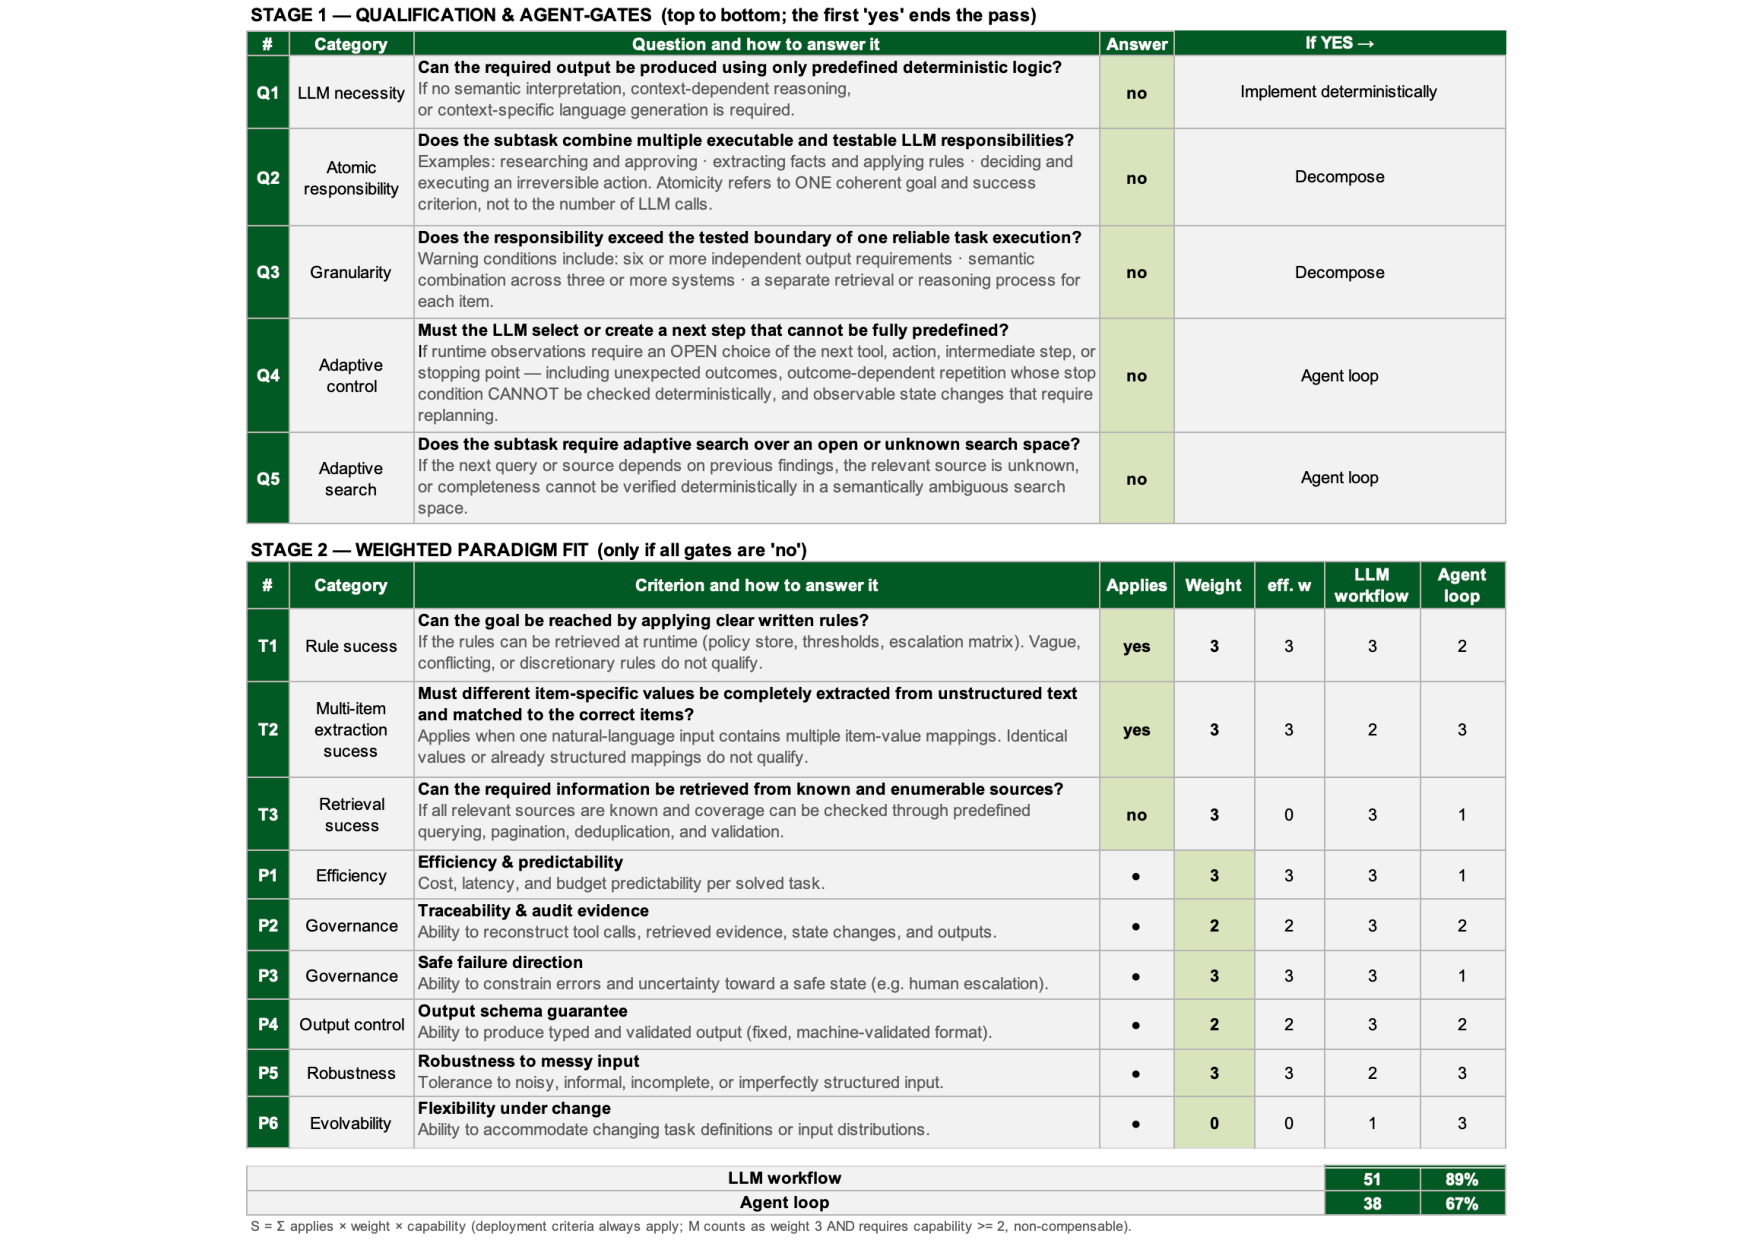
\includegraphics[width=\linewidth,trim=118 2 118 4,clip]{Figures/Initial_Framework_Excel.pdf}
\caption[The initial Decision Sheet]{The initial Decision Sheet (TADF v2.2) in Excel. The architect enters answers and weights in the green cells. \emph{agent loop} denotes the agent. The example applies T1 and T2. The totals at the bottom are the weighted sums and their share of the maximum score. The capability scores are the initial values: efficiency was later corrected, T3 and T2 were retired, and P6 is derived rather than measured (Section~\ref{subsubsec:TADF/evolution}).}
\label{fig:decision-sheet}
\end{figure}

\subsubsection{Development and Evidence}
\label{subsubsec:TADF/evolution}
\label{subsubsec:TADF/evidence}
The first difficulty was the structure of the framework. After the main experimental comparison, TADF v1 was drawn in four forms on 15 and 16 July 2026 (Appendix~\ref{app:evolution/development}). They were an ordered list of routing questions, a strict decision tree with one task dimension per level, a process view and a decision table. The tree did not hold: in the deep-dive runs of X, the suitable orchestration paradigm for rule-generated, record-specific updates depended on the model. The decision table mixed conditions that fix the route with better choices and preferences, and it computed no result. The Decision Sheet therefore became a list with two stages. The gates capture conditions that decide the route regardless of preferences, and the weighted scoring lets the architect set individual priorities. Within Stage 1, the qualification questions come first, because a task that needs no LLM or is too large should not be routed as it stands.

Q1 and Q2 came from a structured self-review of trial applications. Q1 reflects the scope of the evidence: only executions with an LLM were tested, so the framework helps only where a task needs an LLM. Tasks that predefined logic can solve therefore leave the sheet with a deterministic implementation. Q2 fixes the unit of assessment. Each pass assesses one task with one goal and one success criterion; otherwise, it would be unclear during the walkthrough whether the right unit is being assessed.

Q3 addresses tasks that are too large for one execution. At the high level of H, a draft had to meet six or seven constraints over two feedback rounds; at the high level of B, one result had to combine CRM, mail and calendar. Both orchestration paradigms stayed below 60 percent there, and no model exceeded this value (Tables~\ref{tab:app-difficulty-results} and~\ref{tab:app-high-model-results}). This may be related to the number of simultaneous requirements and systems, so Q3 recommends decomposition beyond the warning conditions drawn from these levels. The third warning condition, a separate retrieval or reasoning process for each item, rested on an F task instance with a defective outcome check; it therefore lacks a valid basis (Appendix~\ref{app:evolution/evidence}). Record volume alone did not qualify: in L, more records raised token cost without lowering success (Table~\ref{tab:deepdive-results}).

Q4 selects the agent when the next step depends on what happens during execution. In the three F task instances whose later actions depended on earlier outcomes, the agent solved 13 of 15 executions and the LLM workflow none (Table~\ref{tab:app-main-contrasts}). The deep-dive runs showed the same pattern for repetition until an outcome, for rules applied to outcomes and for observable state changes (P-b, X-1 and M-1 in Table~\ref{tab:deepdive-results}). The LLM workflow plans its actions before it sees their outcomes, so these tasks require an agent. S showed, however, that a state-machine LLM workflow handles outcome branches that are known in advance, so Q4 asks only for an open choice of the next step. Silent state changes defeated both orchestration paradigms (M-2) and therefore became an implementation note, not a gate.

Q5 selects the agent for adaptive search. At the high level of A, a search result determines the next query. There, the agent solved 23 of 25 executions and the LLM workflow 14, and the agent was more successful with every model (Tables~\ref{tab:app-difficulty-results} and~\ref{tab:app-high-model-results}). When the source of a needed fact was unknown (P-c), the agent solved 24 of 25 executions and the LLM workflow 12 (Table~\ref{tab:deepdive-results}).

Stage 2 scores the remaining differences. A task-fit criterion enters only if the two orchestration paradigms fall into different success bands, which are set at 90 and 50 percent. The band then sets the capability score. Table~\ref{tab:initial-evidence} in Appendix~\ref{app:evolution/evidence} gives the basis of each score. Rule success (T1) favors the LLM workflow: with code applying D's written rules, it returned the reference decision in all 75 executions and the agent in 60 (Table~\ref{tab:grid-results}). Extraction success (T2) and retrieval success (T3) rested on the confirmation test and on a development result of B. Among the deployment indicators, the LLM workflow scores higher on efficiency, because the agent used more tokens per success in six task archetypes (Table~\ref{tab:app-token-results}). It also scores higher on safe failure, because twelve of the agent's fifteen incorrect decisions in D were less restrictive than required. Traceability and schema guarantee favor the LLM workflow, whose traces and typed outputs follow from its construction. The agent scores higher on robustness to messy input, based on B's perturbation variants (Table~\ref{tab:app-robustness-results}), and on evolvability, which was derived rather than measured. At the bottom of the sheet, one total per orchestration paradigm summarizes this scoring for the priorities of the architect.

Version 2.2 fixed these rules. Before the freeze, mechanical checks confirmed that the rules return a result for every combination of gate and applicability answers. They also reproduced the expected routes of 49 reference and development cases (Appendix~\ref{app:evolution/verification}). The bands, weights and warning conditions remain design choices, not estimated probabilities. Later audits corrected three elements. The declared efficiency median of 3.6 did not reproduce; the eight task archetypes give 2.21 (Table~\ref{tab:app-token-results}). T3's development result was not reproduced by the main experimental comparison. The task instance behind T2 gives all nine records the same value, so the confirmation test did not measure item-specific values. T3 and T2 were therefore retired before submission (Section~\ref{subsubsec:TADF/artifact-correction}).

\subsubsection{Retrospective Routing Comparison}
\label{subsubsec:TADF/functionality}
A retrospective comparison on the development data gives a first indication of routing value (O5). It applies the archived group-level routes of the Decision Sheet to 17 result groups from the main experimental comparison and the deep-dive runs, with 710 execution slots per strategy (Figure~\ref{fig:routing-value}). The references are always agent, always LLM workflow, random selection and a group-wise oracle and its opposite, which choose the more and the less successful orchestration paradigm per group. The Decision Sheet matched the success of always agent, 82.5 percent, with 6,832 instead of 12,851 recorded tokens per successful execution. Compared with always agent, its routes lost 21 successful executions in B, C, L, S-1 and S-2 and gained 21 in D and E. The oracle was 3.0 percentage points more successful.

\begin{figure}[htbp]
\centering
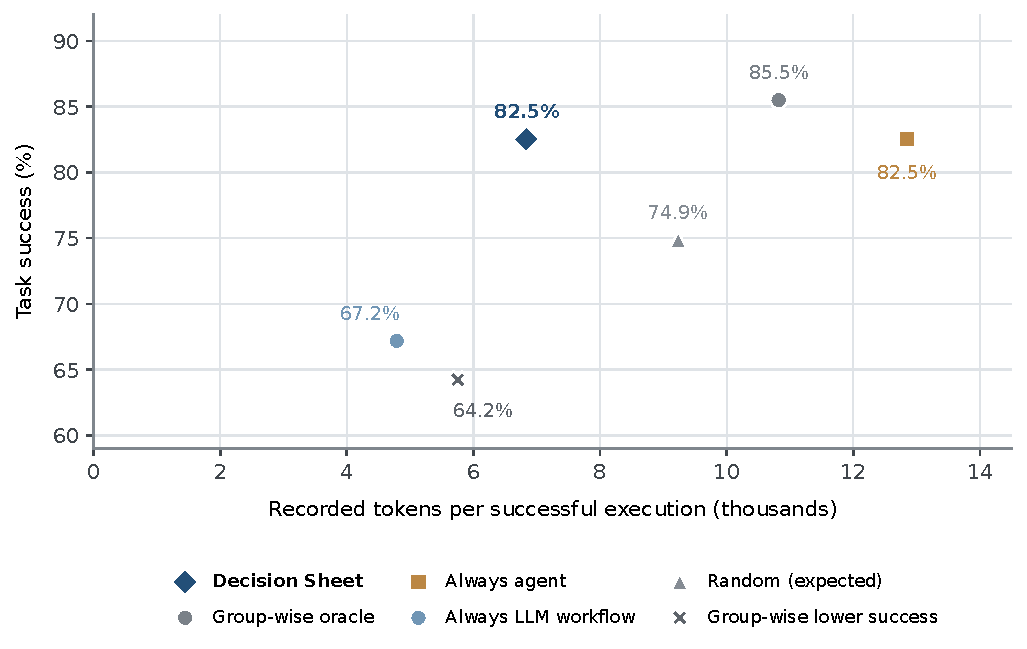
\includegraphics[width=0.8\linewidth]{Figures/fig_routing_value.pdf}
\caption[Retrospective Routing Comparison.]{Retrospective Routing Comparison. Task success and recorded tokens per successful execution of six routing strategies on the development data. Each strategy covers 710 execution slots in 17 result groups. The LLM workflow side includes the state-machine LLM workflow on S-1 and S-2. Costs use the available token observations.}
\label{fig:routing-value}
\end{figure}

The comparison is retrospective. Its groups and routes come from the data that shaped the rules, and the routes apply to groups rather than to single tasks. Repeated executions of a task instance are also not independent. It indicates routing value on the development data only; the evaluation in Section~\ref{subsec:TADF/evaluation} examines the framework beyond them. Appendix~\ref{app:evolution/portfolio} specifies the groups and the calculation.
\FloatBarrier

\subsection{Evaluation}
\label{subsec:TADF/evaluation}
Two evaluation episodes assessed TADF against the design objectives in Section~\ref{subsec:TADF/objectives}. In Episode~1, practitioners described their decision practice and judged the initial Decision Sheet. In Episode~2, the revised framework gave recommendations for WorkBench, and routed execution was compared with using one orchestration paradigm for all tasks. Both episodes led to revisions, following the iterative evaluation activity of DSRM \parencite{peffersDesignScienceResearch2007}. Each episode therefore reports the evaluated version, the findings and the resulting changes.

\subsubsection{Episode 1: Practitioner Interviews}
\label{subsubsec:TADF/episode1}
Episode~1 addressed SQ3 from the perspective of practitioners (Section~\ref{subsec:intro/scope}). It examined whether the choice between the two orchestration paradigms arises in practice, how it is made today, whether the Decision Sheet is understandable and what should change. The sample therefore aimed at people who face this choice in their own work. The inclusion criterion was hands-on experience in building agentic systems or LLM workflow automations. Twelve participants were recruited through LinkedIn, Fiverr and personal contacts. Seven build or advise on AI automations for clients (P02--P07, P09). The others are two engineers, a marketing entrepreneur, the founder of an AI-adoption consultancy and a specialized student (Appendix~\ref{app:eval1/participants}). Together, they cover settings from small businesses to legal, financial and industrial organizations, as well as workflow platforms and agent tools. They thus make the decision that TADF supports, even where their role is not called software architect.

Between 5 and 17 August 2026, ten participants took part in recorded online sessions with screen sharing, nine in German and one in English. P02 and P03 received the Decision Sheet and the questions and answered in writing. A semi-structured guide gave all interviews a common structure: main questions with optional follow-up questions that allowed open answers \parencite{myersQualitativeInterviewResearch2007}. Its five blocks covered the participant's role, a short presentation of the research, the current decision practice, a walkthrough of the Decision Sheet and an open closing question (Appendix~\ref{app:eval1/guide}). P02 and P03 also applied the sheet to a task from their practice. Each interview or written response was anonymized and condensed into a structured record that follows the blocks of the guide. The records keep the participants' statements apart from the interviewer's input and from analytic notes. They were compared in four categories taken from the guide: the relevance of the choice, the current decision practice, the understanding and logic of the Decision Sheet, and improvements. The participant IDs refer to the records in the repository (Appendix~\ref{app:repository}).

The interviews confirmed that the choice arises in practice. All twelve participants described it from their own projects. P02 reported that it comes up increasingly in client discussions. P06 reported clients who ask for an agent because the term is popular, although a simpler solution would suffice. P12 considered the task level relevant because larger automations contain parts with different requirements. P11 also saw the problem as relevant but questioned whether LLM workflows and agents can always be separated cleanly.

In current practice, the choice rests on experience. Ten participants made it by experience, intuition, client preference or platform defaults, without a formal method (P01, P02, P04--P10, P12). Their rules of thumb were similar. A predictable sequence with known outputs led to an LLM workflow. A next step, source or output that could not be listed in advance led to an agent (P02, P03, P06, P07). Four participants kept agents to bounded parts of a workflow (P02--P04, P09), and P10 turned validated agent solutions into reusable workflows. Irreversible actions required deterministic control or human approval (P02, P03, P12). Data protection or approved platforms could rule out a design (P07, P11), and cost was a main criterion for P08, P09 and P12. No record describes a procedure that combines task characteristics, comparative evidence, constraints and priorities. This supports the research gap in Section~\ref{subsec:intro/problem}: the choice recurs in practice, but it rests on rules of thumb.

The Decision Sheet was largely understood. Eight participants found the two stages, gates before a weighted comparison, understandable or consistent with their experience (P01--P04, P06, P08--P10). P01 especially supported the first question, which routes a task to deterministic code if no LLM is needed, and P07 considered both agent gates plausible. P02 and P03 applied the sheet to lead-handling tasks. In both cases, it favored an LLM workflow, which matched their production design or expectation. For P03, the LLM workflow scored 47 and the agent 32 of 51 points, and the mandatory safe-failure marking excluded the agent. P02's production system still passed unclear messages, about one fifth, to a bounded agent step. Unclear points concerned the unit of assessment in Q2 (P02, P03), the basis of the warning conditions in Q3 (P03, P07) and the meaning of Q4 (P02, P03, P11). P01 questioned the schema advantage of the LLM workflow, and P07 found labels and totals hard to read and warned against double counting. The agreement came after the interviewer had explained the sheet, so it shows perceived plausibility rather than independent validation.

The suggested improvements concerned the form of the framework, its scope and its rules. The redesign to TADF v3 adopted the following changes. Table~\ref{tab:eval1-improvements} lists all suggestions, including those not adopted, with the reasons. First, the spreadsheet did not fit how the participants work. Half of them already plan or build automations with LLM assistants or coding agents (P04--P07, P11, P12). Several did not want to fill in a separate spreadsheet for every decision (P04, P08, P11, P12), and the sheet took time or was dense (P01, P05). Participants asked for guided use (P04, P07) or supported an LLM assistant or skill that they could use directly in their work (P05, P06, P08, P11, P12). TADF v3 is therefore delivered as a skill for an LLM assistant. This form also aims at the objective of bounded effort (O7).

Second, metrics’s like task success and token cost alone did not decide the choice. Participants named the environment, such as client requirements, approved platforms, existing tools, data protection, hosting and the people who maintain the solution (P03--P07, P09, P11). They also named the goal of the system. P10 asked whether it should improve through feedback or run a stable procedure, and P11 whether it should assist experts or automate fully. The lifecycle of the system mattered as well, from one-off use to recurring operation and from a prototype to production (P04, P09, P12). The redesign therefore captures the objective and lifecycle of the system before the tasks are assessed. Each recommendation for an LLM workflow or agent also includes checks of the environment.

Third, the distinction and its evidence had to be explained. Several participants asked what exactly separates an LLM workflow from an agent, or used the terms in other ways (P01, P05, P11). Explanations with examples were seen as helpful (P03, P06, P07), and P07 wanted to see the evidence behind a recommendation and the answers that decided it. TADF v3 therefore contains definitions of both orchestration paradigms with measured examples, which the architect can ask about. It also names the evidence behind each recommendation and documents the answers in a decision record (P04, P06, P07, P11, P12). Fourth, participants needed guidance after the route: how to build the chosen design and which safeguards it needs (P09--P11). They named loop limits, logging, output validation and an independent verifier (P01, P02, P08, P10, P12). Each recommendation for an LLM workflow or agent now includes this design knowledge.

Fifth, hard limits and preferences were separated. Irreversible actions needed human approval (P02, P03, P10, P12), and a weighted score should not offset this requirement (P02, P03). A consequential action without a tested rollback therefore requires human approval on every route. Cost and latency are treated separately because their importance differs (P07, P09). The fixed capability scores are kept apart from the architect's weights to avoid double counting (P07). Build effort stays outside the scoring, because coding agents have reduced the effort of building workflows (P04, P07). Finally, the gates were renamed G1--G5, and their questions were sharpened where participants had found them unclear (P02, P03, P06, P07, P11). The framework also states that only the ReAct agent was measured and that the choice of model can change the result (P01, P09, P12).

\subsubsection{Episode 2: WorkBench Evaluation}
\label{subsubsec:TADF/episode2}
\label{subsubsec:TADF/pilots}
Episode~2 addressed the second part of SQ3 (Section~\ref{subsec:intro/scope}). It examined whether TADF gives the same recommendations in two separate passes and whether following them leads to successful execution at low token cost. The test setting was WorkBench, a benchmark of workplace tasks in five domains, such as email and calendar \parencite{stylesWorkBenchBenchmarkDataset2024}. Its 690 task instances come from 69 templates with ten task instances each. A task instance is solved if the resulting database state matches a reference state. The evaluation used the 2026 release WorkBench Revisited, which corrected scoring, reference outcomes and prompts \parencite{stylesWorkBenchRevisitedWorkplace2026}.

WorkBench was selected because both orchestration paradigms could be built on it as this thesis defines them, with the same task instances, tools and scoring (Section~\ref{subsec:theory/workflows-agents}). Its limits were known in advance. All information lies in known databases and the set of tools is fixed, which favors predefined control. A preliminary classification had already expected an LLM workflow for all 69 templates, and open-ended search is hardly covered. WorkBench was still suitable. It tests whether the expected fit leads to more successful and cheaper execution than an agent achieves, and whether the recommendations are stable. It cannot show whether TADF selects an agent where one is needed.

The frozen TADF v3 skill was run for each of the 69 templates, because the ten task instances of a template share one structure (Appendix~\ref{app:eval2/routing}). It received only the template text and a neutral description of the environment. In its benchmark mode, G1--G3 were recorded but could not stop or split a task, so G4, G5 and the comparative assessment chose between the LLM workflow and the agent. The routing ran in two passes of six new sessions each, and the second pass reversed the order of the templates. The recommendations were saved before the evaluation runs began.

All executions used GPT-5.4-mini. The LLM workflow had the two-stage form of task archetype F (Section~\ref{subsubsec:TADF/paradigms}): model calls planned the reads and the actions, and code ran the reads and validated and executed the actions. The agent was the benchmark's own agent, used unmodified in four configurations, and its setup nearly reproduced the published result for this model (Appendices~\ref{app:eval2/freeze} and~\ref{app:eval2/results}). TADF-routed execution was compared with using one orchestration paradigm for all task instances (Always workflow, Always agent). Two strategies were computed from the executions: Random picks an orchestration paradigm per task instance with equal probability, and Oracle picks the agent only where the agent alone succeeds. Besides task success, the evaluation counted side-effect errors, that is, unsuccessful executions that changed records, and mean tokens per task instance, which were estimated from transcripts for the agent (Appendix~\ref{app:eval2/cost}).

Both passes recommended an LLM workflow for all 69 templates, and no gate fired. TADF-routed execution was therefore identical to Always workflow. The input stated no priorities, and the benchmark mode gives each deployment indicator the default weight of 2 unless the template text reveals its weight. Under such a neutral profile, the fixed capability scores favor the LLM workflow by more than the only agent-favoring task-fit criterion can offset. Only G4 or G5 can then select an agent. The agreement concerns the final recommendations, not every answer behind them.

In the first comparison (2a), LLM workflow v1 solved 287 of the 690 task instances (41.6\%). This was below all four agent configurations and matched the main experimental comparison, in which the agent was also more successful in action execution (Section~\ref{subsubsec:TADF/results}). Its best domain was email, the only one with refined prompts. On 50 development task instances from the other domain files, v1 failed 40, mainly because reads depended on earlier results, search parameters did not fit, per-item actions were missing and conditions were mishandled (Appendix~\ref{app:eval2/revision}). TADF's design knowledge already prescribed a bounded re-plan, per-item calls, a placeholder guard and conditions that fail closed, but v1 had implemented none of them. Version~v2.1 therefore added a bounded round of follow-up reads, a check in code against placeholders and unknown identifiers, and general prompt rules. It was frozen and executed on all 690 task instances with the same recommendations (comparison~2b).

With v2.1, following TADF solved 457 task instances (66.2\%), at 7,299 instead of 3,313 tokens per task instance (Figure~\ref{fig:eval2-contribution}). It exceeded the strongest agent, native tool calling with domain tools (60.9\%), by 37 task instances or 5.4 percentage points at about half its estimated token cost. This lead is uncertain, because the task instances of a template are not independent. When templates are resampled, its 95 percent interval ranges from $-1.4$ to 12.2 points (Appendix~\ref{app:eval2/limits}). The gain from v1 to v2.1, 24.6 points with an interval from 16.8 to 32.8, is clear. Random reached 63.6\%. Oracle reached 75.9\%, because the agent solved 67 task instances that v2.1 failed. Choosing in hindsight the better orchestration paradigm for each template would have reached 73.2\%. In comparison~2b, TADF-routed execution thus achieved higher success than Always agent in all four configurations, but it equaled Always workflow. The episode shows no benefit of routing itself.

\begin{figure}[htbp]
\centering
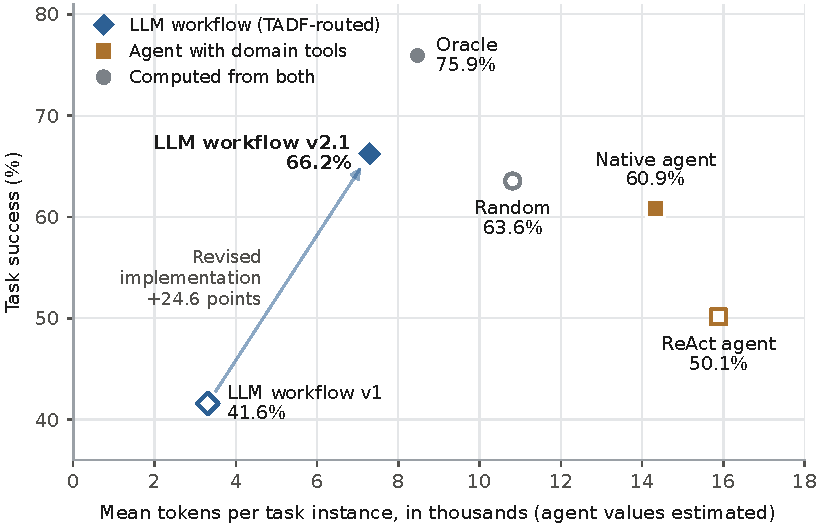
\includegraphics[width=0.94\linewidth]{Figures/fig_workbench_success_tokens.pdf}
\caption[Task success and mean tokens on WorkBench]{Task success and mean tokens per task instance on WorkBench with GPT-5.4-mini. Random and Oracle combine LLM workflow v2.1 with the native agent.}
\label{fig:eval2-contribution}
\end{figure}

Two findings matter for the thesis. First, the benefit of the same recommendations depended on whether the build followed the design knowledge. The revision changed several mechanisms at once, so the effect of single rules remains open. Second, predefined control did not prevent side-effect errors. v2.1 caused 119, fewer than v1 (148) and the native agent (134), but twice as many as the ReAct agent with domain tools (59). TADF's higher safe-failure score for the LLM workflow (P2) assumes a failure direction fixed by design, whereas v2.1 checked conditions and item counts only through its prompts.

The 60 task instances used for development remain among the 690. Without them, v2.1 reached 64.9 percent and the native agent 60.0 percent (Appendix~\ref{app:eval2/limits}). These 630 are still no independent test set, and each configuration has one result per task instance. The results therefore describe the tested implementations on this benchmark (Section~\ref{subsec:discussion/limitations}).

The episode led to three revisions of TADF (Appendix~\ref{app:eval2/framework-revision}). Because some searches return at most five records, G4 now asks whether the planned reads can show all information that the decision needs. If they cannot, G4 fires. Every LLM workflow recommendation now names a mandatory minimum: a bounded re-plan, a placeholder guard, per-item calls with a count check, conditions that fail closed and a pilot before the build is frozen. The architect confirms that the build will implement it. Otherwise, the recommendation stays conditional. Capability scores and weights stayed the same, and the new G4 question was not tested again on WorkBench. Two simulated pilot consultations then refined the dialogue, for example by confirming proposed gate answers together (Appendix~\ref{app:eval2/pilots}).